
\def\layersep{1.8cm}
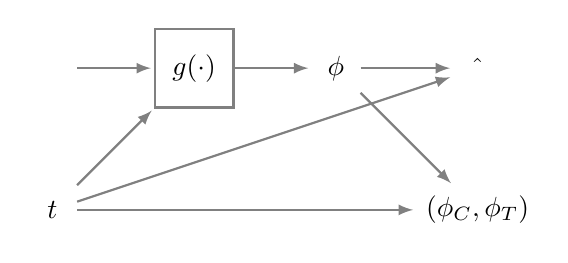
\begin{tikzpicture}[->,>=latex,shorten >=1pt, thick,draw=black!50, node distance=\layersep]

    \tikzstyle{every pin edge}=[<-,shorten <=1pt]
    \tikzstyle{box}=[rectangle,minimum width=1.0cm,minimum height=1.0cm,draw=black!50];
    \tikzstyle{noline}=[box, fill=black!0, minimum width=0.6cm,minimum height=0.6cm, draw=black!0]];
    %\tikzstyle{input neuron}=[box, fill=green!15];

    % Draw the representation node
    \node[noline] (input) at (0,0) {$\bx$};
    \node[box, right of=input] (transform) {$g(\cdot)$};
    \node[noline, right of=transform] (rep) {$\phi$};
    \node[noline, below of=input] (group) {$t$};
    \node[noline, right of=rep] (output) {$\hat{\by}$};
    \node[noline, below of=output] (dist) {$\imb(\phi_C, \phi_T)$};
    %\node[hidden neuron] (lstm-1) at (\layersep,0) {$\bc_0$};
    %\node[output neuron, above of=lstm-1] (output-1) {$\bh_0$};

    \path (input) edge (transform);
    \path (transform) edge (rep);
    \path (rep) edge (output);
    \path (rep) edge (dist);
    \path (group) edge (output);
    \path (group) edge (dist);
    \path (group) edge (transform);
\end{tikzpicture}
